\chapter{Keras: Diseño y desarrollo de modelos}
\lsection{Problema de diabetes - Regresión logística}
Como primer ejemplo introductorio a las redes neuronales en Keras, se va a utilizar un conocido dataset que representa diabetes en indios americanos. Este dataset se puede adquirir en el repositorio de UCI Machine Learning, y describe información médica de pacientes indios, así como información sobre si han tenido diabetes en los siguientes 5 años.\\
La información médica especificada es la siguiente:
\begin{itemize}[noitemsep]
\item Número de embarazos.
\item Concentración de glucosa.
\item Presión en sangre.
\item Tamaño de la doblez de la piel en el triceps.
\item Insulina
\item Índice de masa corporal
\item Función que representa el numero de antepasados con diabetes.
\item Edad
\end{itemize}
\subsection{Cargando datos}
Cuando se trabaja con algoritmos de Machine Learning que usan números aleatorios, es una buena metodología de trabajo predefinir de antemano una semilla. Con ello, podremos ejecutar el mismo código varias veces obteniendo el mismo resultado. Esta idea es bastante útil a la hora de demostrar un resultado, comparar distintos algoritmos, debuggear parte del código...\\
Se iniciará la generación de números aleatorios con la semilla que queramos, por ejemplo:
\begin{lstlisting}[language=Python]
from keras.models import Sequential
from keras.layers import Dense
import numpy
numpy.random.seed(4)
\end{lstlisting}
Nos encontramos ante un problema de clasificación binaria (tener diabetes representa salida 1, y no tenerla salida 0). Todas las variables que definen al paciente son numéricas, lo cual hace fácil su uso directamente en redes neuronales, que esperan datos numéricos tanto en las entradas como en las salidas.\\
Una vez que tenemos descargado nuestra fuente de datos, podremos cargarla directamente usando la funcion \lstinline{loadtxt()} de la libreria NumPy. En este dataset, podemos apreciar 8 datos de entrada, y 1 variable de salida (la última columna). Una vez cargado, podemos separar los datos en variables de entrada y targets.
\begin{lstlisting}[language=Python]
dataset = numpy.loadtxt("pima-indians-diabetes.csv", delimiter=",")
X = dataset[:,0:8]
Y = dataset[:,8]
\end{lstlisting}

\subsection{Definiendo el modelo}
Como se ha comentado en el capítulo 3, los módelos en Keras se definen como una secuencia de capas. La primera cosa de la que hay que asegurarse, es de que la capa de entrada tiene el número correcto de entradas. Esto se define mediante el argumento \lstinline{input_dim}, cuando se crea la primera capa.\\
Las capas totalmente conectadas se definen usando la clase \lstinline{Dense}. Podemos especificar el número de neuronas de la capa utilizando el primer argumento, el método de inicialización con el segundo (\lstinline{init}), y la función de activación usando el argumento \lstinline{activation}.\\
En este caso, se inicializarán los pesos de la red con pequeños números aleatorios de una distribución Gaussiana (\lstinline{normal}). Se usará la función de activación rectificadora (\lstinline{relu}) en las primeras dos capas, y la función sigmoide en la capa de salida. Las funciones sigmoide e hiperbólica solían ser las funciones de activación más utilizadas. Sin embargo, a día de hoy, se consiguen mejores resultados utilizando la función de activación rectificadora. La función sigmoide en la capa de salida será necesaria para asegurarse que la salida de nuestro modelo comprende valores entre 0 y 1.\\
La primera capa tendrá 12 neuronas y espera 8 variables de entrada. La segunda tiene 8 neuronas, y la ultima solo 1, la cual reflejará en su salida la predicción sobre si para los datos médicos introducidos como entrada, se tendrá diabetes o no.
\begin{lstlisting}[language=Python]
model = Sequential()
model.add(Dense(12, input_dim=8, init='normal', activation='relu'))
model.add(Dense(8, init='normal', activation='relu'))
model.add(Dense(1, init='normal', activation='sigmoid'))
\end{lstlisting}

\subsection{Compilando el modelo}
Una vez que se ha definido el modelo, el siguiente paso es compilarlo. Aquí es donde entra en juego el backend elegido (Theano o Tensorflow), ya que Keras utiliza sus librerías numéricas. El propio backend es el encargado de elegir la mejor forma para entrenar la red y de hacer predicciones con ella, utilizando la CPU, la GPU o ambas a la vez.\\
En la fase de compilación, se deben especificar algunas propiedades adicionales para entrenar la red (recordar que entrenar una red significa encontrar los mejores pesos para hacer predicciones de un problema). Debemos especificar la función de perdida para evaluar los pesos, el optimizador usado para elegir entre los diferentes pesos, y métricas opcionales para recoger y mostrar los datos durante el entrenamiento.\\
En este ejemplo, se utilizará una función de perdida logarítmica, que para los problemas de clasificación está definida en Keras como \lstinline{binary_crossentropy}. Como optimizador se utilizará el algoritmo de gradiente descendiente \lstinline{adam}, el cual usa Keras por defecto.\\
Finalmente, como se trata de un problema de clasificación, se recogerá y mostrará la eficiencia de la clasificación, o lo que es lo mismo, el porcentaje de aciertos (argumento \lstinline{accuracy}).

\begin{lstlisting}[language=Python]
model.compile(loss='binary_crossentropy', optimizer='adam', metrics=['accuracy'])
\end{lstlisting}

\subsection{Ajustando el modelo}
Una vez compilado, el siguiente paso es ejecutar el modelo con los datos de entrada. Podemos entrenar o ajustar nuestro modelo cargando los datos utilizando la función \lstinline{fit()}.\\
El proceso de entrenamiento se ejecutará para un número de iteraciones definido mediante el argumento \lstinline{nb_epoch}. También podemos definir el numero de entradas que serán evaluadas antes de que haya una actualización de los pesos de la red mediante el argumento \lstinline{batch_size}). De nuevo, estas medidas pueden ser elegidas experimentalmente a base de prueba y error.
\begin{lstlisting}[language=Python]
model.fit(X, Y, nb_epoch=150, batch_size=10)
\end{lstlisting}

\subsection{Evaluando el modelo}
Una vez entrenada la red neuronal, podemos evaluar el rendimiento de esta utilizando el mismo dataset. Esto nos puede dar una idea de cómo hemos modelado los datos de entrada, pero no tendremos idea de como de bien clasificará los nuevos datos nuestro modelo.\\
Para evaluar nuestra red, se utiliza la función \lstinline{evaluate()}. En este ejemplo, se le pasarán las mismas entradas que cuando se entrenó la red, generando así una predicción por cada par de entrada-salida, además de mostrar información sobre las la perdida media y la precisión de nuestro modelo.
\begin{lstlisting}[language=Python]
eva = model.evaluate(X, Y)
print("%s: %.2f%%" % (model.metrics_names[1], eva[1]*100))
\end{lstlisting}

\subsection{Analizando datos}
Al ejecutar el código, podemos ver un mensaje por cada 150 ciclos mostrando la pérdida y la precisión de cada uno, seguido de los resultados finales.
\begin{lstlisting}
Epoch 1/150
768/768 [==============================] - 0s - loss: 0.6829 - acc: 0.6471
Epoch 2/150
768/768 [==============================] - 0s - loss: 0.6654 - acc: 0.6510
Epoch 3/150
768/768 [==============================] - 0s - loss: 0.6556 - acc: 0.6510
...
Epoch 148/150
768/768 [==============================] - 0s - loss: 0.4487 - acc: 0.7826
Epoch 149/150
768/768 [==============================] - 0s - loss: 0.4444 - acc: 0.7839
Epoch 150/150
768/768 [==============================] - 0s - loss: 0.4456 - acc: 0.7747
 32/768 [>.............................] - ETA: 0
 sacc: 77.34%
\end{lstlisting}
El siguiente paso es adaptar el ejemplo anterior y utilizarlo para generar predicciones sobre el dataset de entrenamiento, simulando que nos encontramos ante un nuevo dataset que nunca hemos analizado previamente. Mediante la función \lstinline{model.predict}, podremos realizar estas predicciones fácilmente.\\
Con las siguientes lineas, se mostrarán predicciones para cada entrada del dataset, que en su mayor parte, coincidirán con los datos de salida ya descritos en el dataset. Recordar que 1 es padecer diabetes, y 0 lo contrario.
\begin{lstlisting}[language=Python]
predicciones = model.predict(X)
rounded = [round(x) for x in predicciones]
print(rounded)
\end{lstlisting}

\clearpage
\lsection{Problema Boston Housing - Regresión lineal}
\subsection{Descripcion del problema}
En este caso, nos encontramos ante un problema de regresión lineal. El dataset describe 13 propiedades numéricas de 506 casas de los suburbios de Boston, con el precio de dichas casas en millones de dolares. Este conocido dataset puede ser adquirido en el repositorio de UCI Machine Learning. Como atributos de entrada, disponemos de:
\begin{itemize}[noitemsep]
\item CRIM: ratio de crimen per capita por población.
\item ZN: proporción de tierras residenciales zonificadas con más de 25000 pies cuadrados.
\item INDUS: proporción de acres no comerciales por ciudad
\item CHAS: Charles River dummy variable ( 1 si el tramo se encuentra en el río, 0 en caso contrario).
\item NOX: concentración de óxidos nítricos.
\item RM: numero medio de habitaciones por vivienda.
\item AGE: proporción de viviendas ocupadas construidas antes de 1940.
\item DIS: distancias ponderadas a cinco centros de empleo.
\item RAD: índice de accesibilidad a las autopistas radiales.
\item TAX: ratio de impuestos a la propiedad por cada 10.000\$.
\item PTRATIO: ratio de alumnos-profesores.
\item B: ${1000(Bk - 0.63)^2}$ donde Bk es la proporción de ciudadanos negros por población.
\item LSTAT: porcentaje de la población de clase baja.
\end{itemize}
Como target, nos proporcionan el valor medio de las casas ocupadas, en miles de dolares.\\
Un rendimiento razonable en modelos actuales usando el Error cuadrático medio (MSE) como método de evaluación está en torno a 20 (miles de dolares al cuadrado). Veamos si podemos igualar estos resultados.
\subsection{Desarrollo de la red neuronal}
Lo primero, será cargar todas las librerías necesarias, así como el dataset.
\begin{lstlisting}[language=Python]
import numpy
import pandas
from keras.models import Sequential
from keras.layers import Dense
from keras.wrappers.scikit_learn import KerasRegressor
from sklearn.model_selection import cross_val_score
from sklearn.model_selection import KFold
from sklearn.preprocessing import StandardScaler
from sklearn.pipeline import Pipeline

dataframe = pandas.read_csv("housing.csv", delim_whitespace=True, header=None)
dataset = dataframe.values

X = dataset[:,0:13]
Y = dataset[:,13]
\end{lstlisting}
En este ejemplo se crearán modelos en Keras, y serán ajustados y evaluados utilizando la librería Scikit-learn. Esta librería Python open source de Machine Learning es bastante potente a la hora de evaluar modelos con pocas lineas de código.\\
El siguiente paso por tanto es crear el modelo de la red neuronal. Para el problema Boston-Housing basta con diseñar un modelo de red con una sola capa oculta totalmente conectada con el mismo numero de neuronas que de entradas (13). Como función de activación en la capa oculta se usa la función rectificadora. Para la capa de salida no se usa ninguna función de activación debido a que nos encontramos ante un problema de regresión, y el objetivo es predecir valores numéricos directamente sin aplicarles ningún tipo de transformación. Como algoritmo de optimización usaremos \lstinline{adam}, y como función de perdida el error cuadrático medio. Estas métricas también serán usadas para evaluar el rendimiento del modelo. Se ha elegido esta métrica ya que al usar la raíz cuadrada, se nos presenta un valor de error directamente entendible en el contexto del problema (miles de dolares).
\begin{lstlisting}[language=Python]
def baseline_model():
	model = Sequential()
	model.add(Dense(13, input_dim=13, init='normal', activation='relu'))
	model.add(Dense(1, init='normal'))
	model.compile(loss='mean_squared_error', optimizer='adam')
	return model
\end{lstlisting}
El wrapper de Keras para usar Scikit-Learn como un estimador de regresión se llama KerasRegressor. Podemos crear una instancia y pasarle como argumentos:
\begin{enumerate}[noitemsep]
\item El nombre de la función que define la red neuronal (\lstinline{baseline_model()})
\item Parámetros que se le pasarán a la funcion \lstinline{fit()}, como el número de ciclos o el tamaño de los lotes.
\end{enumerate}
Como siempre, además se debe inicializar una semilla aleatoria constante para asegurarnos que la comparación de los modelos es consistente.
\begin{lstlisting}[language=Python]
numpy.random.seed(4)
estimator = KerasRegressor(build_fn=baseline_model, nb_epoch=100, batch_size=5, verbose=0)
\end{lstlisting}
El siguiente paso es evaluar el modelo. Para ello, se usará una validación cruzada de 10 iteraciones.
\begin{lstlisting}[language=Python]
kfold = KFold(n_splits=10, random_state=seed)
results = cross_val_score(estimator, X, Y, cv=kfold)
print("Resultados: %.2f (%.2f) MSE" % (results.mean(), results.std()))
\end{lstlisting}
Ejecutando todo el código veremos una estimación del rendimiento del modelo. El resultado muestra el error cuadrático medio incluyendo la media y la desviación típica a lo largo de las 10 iteraciones de la evaluación por validación cruzada.
\begin{lstlisting}
Resultados: 31.35 (25.45) MSE
\end{lstlisting}
\subsection{Mejorando los resultados}
Aunque ya hayamos conseguido entrenar nuestra red para obtener resultados, existen muchas maneras de mejorar nuestro modelo. En este ejemplo, veremos tres:
\begin{itemize}[noitemsep]
\item Normalizar el dataset de entrada
\item Aumentar el numero de capas
\item Aumentar el numero de neuronas en las capas
\end{itemize}
\subsubsection{Normalizando el dataset}
Un factor muy importante en el dataset de Boston-housing es que los atributos de entrada varían mucho sus escalas, ya que miden cantidades diferentes. Por este tipo de razones, siempre suele ser una buena práctica preparar los datos antes de modelarlos usando nuestra red neuronal.\\
Para ver la diferencia con esta mejora, se va a usar el mismo modelo de red neuronal que en el apartado anterior. Se va a usar el framework Pipeline de Scikit-Learn para estandarizar el modelo de datos durante el proceso de evaluación dentro de cada pliegue de la validación cruzada. Esto asegura que no haya datos de nuestro set de entrenamiento sin evaluar en cada pliegue de la validación cruzada.
\begin{lstlisting}[language=Python]
numpy.random.seed(seed)
estimators = []
estimators.append(('standardize', StandardScaler()))
estimators.append(('mlp', KerasRegressor(build_fn=baseline_model, nb_epoch=50, batch_size=5, verbose=0)))
pipeline = Pipeline(estimators)
kfold = KFold(n_splits=10, random_state=seed)
results = cross_val_score(pipeline, X, Y, cv=kfold)
print("Estandarizado: %.2f (%.2f) MSE" % (results.mean(), results.std()))
\end{lstlisting}
En el código anterior, se crea un \lstinline{Pipeline} de Scikit-Learn, donde primero se estandarizan los datos y luego se evalúa el modelo desarrollado en el apartado anterior. Al ejecutar todo el código, vemos una mejora en el rendimiento respecto al modelo sin estandarizar los datos.
\begin{lstlisting}
Estandarizado: 30.78 (29.41) MSE
\end{lstlisting}
\subsubsection{Red neuronal más profunda}
Otra manera de mejorar nuestra red neuronal es añadirle capas, lo cual permitirá al modelo extraer más cantidad de características del dataset.\\
En este apartado se evaluará el efecto de añadir más de una capa al modelo. Ésto es tan fácil como crear una nueva función copia de la anterior, pero insertando nuevas lineas después de la primera capa oculta. En este ejemplo, cada capa tendrá la mitad de neuronas que la capa anterior.
\begin{lstlisting}[language=Python]
def modelo_profundo():
	model = Sequential()
	model.add(Dense(13, input_dim=13, init='normal', activation='relu'))
	model.add(Dense(6, init='normal', activation='relu'))
	model.add(Dense(1, init='normal'))
	model.compile(loss='mean_squared_error', optimizer='adam')
	return model
\end{lstlisting}
Como podemos apreciar, los datos pasarán por una capa de entrada de 13 neuronas, después por una de 6, para acabar en una capa de salida de una sola neurona. La forma de evaluar el modelo será la misma que en el apartado anterior, usando la estandarización de los datos de entrada para mejorar aún más el rendimiento.\\
Ejecutando todo el código podemos ver otra importante mejora en el rendimiento respecto al apartado anterior:
\begin{lstlisting}
Resultados: 24.10 (28.45) MSE
\end{lstlisting}
\subsubsection{Red neuronal más ancha}
Otra forma de incrementar la capacidad de nuestro modelo es crear un red más ancha. En este apartado se evaluará el efecto de añadir a nuestra arquitectura una capa oculta con el doble de neuronas de las que tiene la capa de entrada.\\
De nuevo, se ha de definir una nueva función como en los ejemplos anteriores, pero que cuente con una capa oculta entre la capa de entrada y la de salida de 20 neuronas.
\begin{lstlisting}[language=Python]
def modelo_ancho():
	model = Sequential()
	model.add(Dense(20, input_dim=13, init='normal', activation='relu'))
	model.add(Dense(1, init='normal'))
	model.compile(loss='mean_squared_error', optimizer='adam')
	return model
\end{lstlisting}
Como podemos ver, nuestros datos pasarán de una capa de entrada de 13 neuronas, a una capa oculta de 20, para luego acabar en una capa de salida de una sola neurona. De nuevo, la forma de evaluar el modelo será la misma que en los dos apartados anteriores, usando la estandarización de los datos de entrada para mejorar el rendimiento.\\
Ejecutando el código podemos ver una mejora aún mayor que la que se consiguió con la red neuronal más profunda. No es nada mal resultado para este tipo de problema:
\begin{lstlisting}
Resultados: 21.66 (24.12) MSE
\end{lstlisting}
Como se ha comentado anteriormente, no es del todo fácil ver que con una red más profunda se consigan mejores resultados en este tipo de problemas. Esto demuestra la importancia de tener que testear varios tipos de modelos, para conseguir así los mejores resultados.

\lsection{MNIST - Perceptrón multicapa vs Red convolucional}
El dataset MNIST fue desarrollado con el objetivo de evaluar modelos de redes neuronales utilizando el problema de clasificación de dígitos escritos a mano. Este dataset esta constituido por un gran número de documentos escaneados por el National Institute of Standards and Technology (NIST), a los cuales se le han extraído y normalizado sus caracteres. Cada imagen es de 28x28 píxeles, y se usan 60.000 imágenes para entrenar el modelo, y otras 10.000 para probarlo.\\
Estamos hablando de una tarea de reconocimiento de dígitos. Al haber 10 dígitos (del 0 al 9), hay 10 clases para clasificar. El estado del arte del error de predicción está en el 0,2\%, que puede ser alcanzado con grandes redes neuronales convolucionales en las que se aplican técnicas avanzadas como DropConnect o aumento de patrones.\\
\subsection{Cargando el dataset}
Mediante la librería Keras, es posible descargarse el dataset de manera automática. Para ello, se llamará a la función \lstinline{mnist.load_data()}, que almacenará la información en el directorio \lstinline{~/.keras/datasets/mnist.pkl.gz}.
\mbox{}
\begin{figure}[htp]
\centering
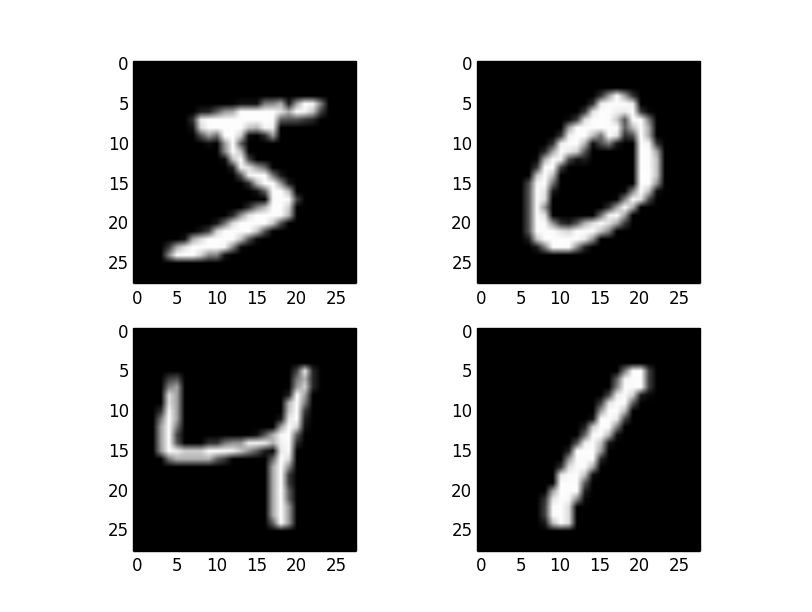
\includegraphics[scale=0.20]{images/mnist.png}
\caption{Patrones dataset MNIST}
\end{figure}
\\No es estrictamente necesaria una red neuronal convolucional para conseguir buenos resultados con el dataset MNIST. Mediante una red neuronal sencilla, con una sola capa oculta, podemos alcanzar un ratio de error del 1.74\%. Se usará este dato como base para comparar más modelos de redes convolucionales más adelante.\\
Lo primero de todo, como ya hemos visto, es cargar los módulos necesarios, generar una semilla aleatoria (aunque fija), y cargar el dataset.\\
El set de entrenamiento está estructurado como un array tridimensional compuesto por la imagen, su ancho y su alto. Para poder utilizarlo con un perceptrón, tenemos que convertir las imágenes en un vector de píxeles. En este caso, las imágenes de 28x28 se convertirán en 748 valores de entrada. Podemos hacer esto fácilmente  con la función \lstinline{reshape()} de NumPy.
\begin{lstlisting}[language=Python]
import numpy
from keras.datasets import mnist
from keras.models import Sequential
from keras.layers import Dense
from keras.layers import Dropout
from keras.utils import np_utils

numpy.random.seed(4)

n_pixels = X_train.shape[1] * X_train.shape[2]
X_train = X_train.reshape(X_train.shape[0], n_pixels).astype('float32')
X_test = X_test.reshape(X_test.shape[0], n_pixels).astype('float32')
\end{lstlisting}

Los valores van de 0 a 255, en una escala de grises. Cuando se trabaja con modelos de redes neuronales, suele ser buena idea escalar o normalizar los datos de entrada. Para ello, se convertirán estos valores del rango 0-255 al 0-1.\\
Además, la salida será un entero entre 0 y 9 (ya que como hemos dicho, tenemos 10 clases en las que nuestra imagen puede ser clasificada). Nos encontramos ante un problema de multiclasificación, por lo que será útil codificar el vector de enteros en una matriz binaria:
\begin{lstlisting}[language=Python]
X_train = X_train / 255
X_test = X_test / 255

y_train = np_utils.to_categorical(y_train)
y_test = np_utils.to_categorical(y_test)
num_classes = y_test.shape[1]
\end{lstlisting}

Con todo esto, ya se puede crear el modelo de la red neuronal. En este ejemplo, vamos a diseñar tanto un modelo de red neuronal basado en un perceptrón multicapa como un modelo convolucional, para ver sus diferencias y rendimientos a la hora de tratar imágenes.
\subsubsection{Perceptrón multicapa}
\begin{lstlisting}[language=Python]
def perceptron_model():
	model = Sequential()
	model.add(Dense(n_pixels, input_dim=n_pixels, init='normal', activation='relu'))
	model.add(Dense(num_classes, init='normal', activation='softmax'))
	model.compile(loss='categorical_crossentropy', optimizer='adam', metrics=['accuracy'])
	return model
\end{lstlisting}
Como podemos observar, se trata de un modelo con una sola capa oculta, con el mismo numero de neuronas que de entradas, es decir, 784. Además, sobre ella se aplica una función de activación rectificadora.\\
En la capa de salida, se usa la función de activación softmax para convertir las salidas en una probabilidad, y permitir que se seleccionen una de las 10 clases que el modelo ha de predecir. Como función de perdida, se utiliza la perdida logarítmica (en Keras, \lstinline{categorical_crossentropy}). Por último, para que la red entrene y aprenda los pesos, se utiliza el algoritmo gradiente descendiente \lstinline{adam}.\\
\subsubsection{Red convolucional}
\begin{lstlisting}[language=Python]
def convolutional_model():
	model = Sequential()
	model.add(Convolution2D(32, 5, 5, init='glorot_uniform', border_mode='valid', input_shape=(1, 28, 28), activation='relu'))
	model.add(MaxPooling2D(pool_size=(2, 2)))
	model.add(Dropout(0.2))
	model.add(Flatten())
	model.add(Dense(128, activation='relu'))
	model.add(Dense(num_classes, activation='softmax'))
	model.compile(loss='categorical_crossentropy', optimizer='adam', metrics=['accuracy'])
	return model
\end{lstlisting}
Como podemos ver, las redes convolucionales son bastante más complejas que los perceptrones multicapa. En resumen, nuestro modelo cuenta con las siguientes capas:\\
\begin{enumerate}
\item La primera capa es una capa convolucional (\lstinline{Convolution2D}). Cuenta con 32 mapeadores, de tamaño 5x5, una función de activación rectificadora, y un inicializador de tipo \lstinline{glorot_uniform} (usado por defecto en las capas convolucionales de Keras) . Al ser la capa de entrada, esperará imágenes con la forma \lstinline{[[píxeles][ancho][alto]]}.
\item Después se define una capa pooling que utilizará la función máximo, con un tamaño de 2x2.
\item La siguiente capa (\lstinline{Dropout}) será regularizadora. Se ha configurado para excluir aleatoriamente el 20\% de las neuronas de la capa y así reducir el sobreajuste.
\item La siguiente capa (\lstinline{Flatten}) convertirá la matriz de 2 dimensiones en un vector, permitiendo de esta forma que la salida pueda ser procesada por una capa totalmente conectada.
\item Después se ha añadido una capa totalmente conectada con 128 neuronas y una función de activación rectificadora.
\item Finalmente, la capa de salida tendrá 10 neuronas, una por cada clase a predecir, y una función de activación softmax para hacer una aproximación de la probabilidad de que cada entrada se corresponda con cada clase (es decir, con cada numero).
\end{enumerate}
Como en el ejemplo del perceptrón multicapa, el modelo se entrenará usando la función de pérdida logarítmica y el algoritmo \lstinline{adam} de gradiente descendiente.
\subsection{Resultados}
Ahora ya podemos ajustar y evaluar los modelos. Estos se ajustán cada 10 ciclos, con actualizaciones cada 200 imágenes. Finalmente, se muestra el ratio de error de clasificación.
\begin{lstlisting}[language=Python]
model = perceptron_model() // model.convolutional_model
model.fit(X_train, y_train, validation_data=(X_test, y_test), nb_epoch=10, batch_size=200, verbose=2)
scores = model.evaluate(X_test, y_test, verbose=0)
print("Baseline Error: %.2f%%" % (100-scores[1]*100))
\end{lstlisting}
Ejecutando todo el código anterior utilizando el modelo del perceptrón multicapa, veremos la siguiente salida. Como podemos observar, esta red neuronal tiene un ratio de error de 1.88\%.
\begin{lstlisting}
Epoch 1/10
10s - loss: 0.2792 - acc: 0.9206 - val_loss: 0.1358 - val_acc: 0.9615
Epoch 2/10
8s - loss: 0.1096 - acc: 0.9681 - val_loss: 0.0917 - val_acc: 0.9720
Epoch 3/10
8s - loss: 0.0704 - acc: 0.9799 - val_loss: 0.0727 - val_acc: 0.9780
...
Epoch 8/10
9s - loss: 0.0152 - acc: 0.9963 - val_loss: 0.0620 - val_acc: 0.9797
Epoch 9/10
10s - loss: 0.0104 - acc: 0.9978 - val_loss: 0.0598 - val_acc: 0.9821
Epoch 10/10
9s - loss: 0.0089 - acc: 0.9980 - val_loss: 0.0640 - val_acc: 0.9812
Classification Error: 1.88%

\end{lstlisting}
Sin embargo, si ejecutamos el código utilizando el modelo convolucional, tendríamos un ratio de error de 1.02\%, y la siguiente salida:
\begin{lstlisting}
Epoch 1/10
162s - loss: 0.2484 - acc: 0.9289 - val_loss: 0.0799 - val_acc: 0.9773
Epoch 2/10
151s - loss: 0.0752 - acc: 0.9777 - val_loss: 0.0519 - val_acc: 0.9833
Epoch 3/10
151s - loss: 0.0531 - acc: 0.9841 - val_loss: 0.0376 - val_acc: 0.9883
...
Epoch 8/10
150s - loss: 0.0191 - acc: 0.9938 - val_loss: 0.0298 - val_acc: 0.9898
Epoch 9/10
156s - loss: 0.0173 - acc: 0.9945 - val_loss: 0.0306 - val_acc: 0.9901
Epoch 10/10
155s - loss: 0.0162 - acc: 0.9949 - val_loss: 0.0323 - val_acc: 0.9898
Classification Error: 1.02%
\end{lstlisting}
Como se puede observar, hemos reducido el error de clasificación del 1.88\% al 1.02\%. Pero... ¿podríamos obtener mejores resultados? La respuesta es sí. En este ejemplo, se ha utilizado una red convolucional muy simple. Sin embargo, añadiendo más capas convolucionales, de pooling y totalmente conectadas, podemos acercarnos a ratios de error muy cercanos al estado del arte actual. Por ejemplo, añadiendo una nueva capa convolucional (\lstinline{model.add(Convolution2D(15, 3, 3, activation='relu')), model.add(MaxPooling2D(pool\_size=(2, 2)))}),y una nueva capa totalmente conectada (\lstinline{model.add(Dense(50, activation='relu'))}), obtendríamos un ratio de error de  0.89\%.

\lsection{Generación de textos - Red LSTM}
\label{ej_lstm}
En este ejemplo, se va a intentar generar textos que más o menos tengan sentido. Hasta la aparición de las redes neuronales, que un ordenador pudiese llevar a cabo esta tarea parecía una idea sacado de una película de ciencia ficción. Sin embargo, con las redes LSTM esto empieza a ser posible.\\
Las redes neuronales, además de ser usadas para predecir modelos, pueden ser utilizadas para aprender secuencias de un problema y generar mediante estos conocimientos nuevas secuencias. Los modelos que generan nuevas secuencias como éste, no solo son útiles para saber como de bien nuestra máquina ha aprendido un problema, sino también para saber más sobre un problema en sí mismo.\\
En este ejemplo, se va a utilizar el libro "La metamorfosis" de Kafka como dataset para nuestra red neuronal. Ésta, va a aprender las dependencias entre los diferentes caracteres que se vaya encontrando a lo largo del texto así como las probabilidades de que estos caracteres aparezcan, con el objetivo de generar una nueva secuencia de caracteres, formando así un nuevo texto y una nueva historia. Sin embargo, este ejemplo también es válido para otro tipo de textos: poemas, código fuente... (siempre que éstos se encuentren en código ASCII).
\subsection{Aprendiendo secuencias de caracteres}
Primero se importan las clases que se van a utilizar en el problema, y se carga el texto convirtiéndolo todo a minúsculas.
\begin{lstlisting}[language=Python]
import numpy
from keras.models import Sequential
from keras.layers import Dense
from keras.layers import Dropout
from keras.layers import LSTM
from keras.callbacks import ModelCheckpoint
from keras.utils import np_utils

filename = "metamorfosis.txt"
raw_text = open(filename).read()
raw_text = raw_text.lower()
\end{lstlisting}
Una vez cargado el libro en memoria, debemos prepararlo para ser tratado por una red neuronal. Una buena idea es convertir los caracteres a números enteros. Para ello, primero se identifican todos los caracteres que componen el texto y se asocia un numero a cada uno. Con ello, se consigue reducir el numero de caracteres a analizar, ya que también se eliminarán los repetidos.
\begin{lstlisting}[language=Python]
chars = sorted(list(set(raw_text)))
char_to_int = dict((c, i) for i, c in enumerate(chars))
\end{lstlisting}
El siguiente paso es definir el conjunto de entrenamiento. Se dividirá el texto en conjuntos de caracteres (en este ejemplo 100), para pasárselos como entrada a la red neuronal. El objetivo es que la red prediga el carácter 101. Esto se conseguirá desplazando de 1 en 1 los 100 caracteres seleccionados, permitiendo así que cada carácter sea aprendido por los 100 caracteres que le preceden. Por ejemplo, si hiciésemos divisiones de 5 en 5, y tuviésemos la palabra CAPITULO, las iteraciones serían:
\begin{lstlisting}
CAPIT -> U
APITU -> L
PITUL -> O
\end{lstlisting}
Dado que las redes neuronales trabajan con números en vez de caracteres, debemos convertir estos caracteres a enteros usando la tabla que generamos anteriormente.
\begin{lstlisting}[language=Python]
seq_length = 100
dataX = []
dataY = []
for i in range(0, n_chars - seq_length, 1):
	seq_in = raw_text[i:i + seq_length]
	seq_out = raw_text[i + seq_length]
	dataX.append([char_to_int[char] for char in seq_in])
	dataY.append(char_to_int[seq_out])
n_patterns = len(dataX)
print "Total Patterns: ", n_patterns
\end{lstlisting}
Si ejecutamos el código hasta este punto, podemos ver el numero de patrones de entrenamiento: \lstinline{121472}\\
Una vez que hemos preparado el dataset, necesitamos transformarlo para que pueda ser usado por Keras. Primero, debemos transformar la lista de entradas (\lstinline{seq_in}) en una secuencia de la forma \lstinline{[muestra, intervalo de tiempo, característica]}, esperada por una red LSTM. Después, se necesita escalar los enteros al rango 0-1 para conseguir patrones más fáciles de aprender por la red LSTM que usa la función de activación sigmoide. Finalmente, se convertirán los patrones de salida. Para ello, se representará la salida como una probabilidad de que aparezca cada uno de los 43 caracteres distintos que componen el texto, en vez de intentar predecir estrictamente el siguiente carácter. Cada valor será convertido a un vector de longitud 43, relleno de 0 menos un 1 que concidirá con la columna de la letra que el patrón representa. Por ejemplo, si la letra fuese la C (entero numero 3), la codificación sería... [0,0,1,0,0,0,0,0...0]
Esto se consigue mediante las siguientes lineas de código.
\begin{lstlisting}[language=Python]
X = numpy.reshape(dataX, (n_patterns, seq_length, 1))
X = X / float(n_vocab)
y = np_utils.to_categorical(dataY)
\end{lstlisting}
Una vez que tenemos los datos preparados, es hora de definir nuestra red LSTM. Para este ejemplo, se definirán dos capas oculta LSTM con 256 unidades de memoria. Se usa la técnica de regularización para evitar el sobreajuste conocida como \lstinline{Dropout}, con una probabilidad del 20\%. La capa de salida será una capa lstinline{Dense} que usará \lstinline{softmax} como función de activación para producir una salida en función de la probabilidad de que aparezca uno de los 43 caracteres.\\
En realidad, podemos observar que el problema es realmente un problema de clasificación con 43 clases, y por ello se define la función de perdida logarítmica \lstinline{cross entropy} y se aplica el algoritmo de optimización \lstinline{adam} para mejorar la velocidad.
\begin{lstlisting}[language=Python]
model = Sequential()
model.add(LSTM(256, input_shape=(X.shape[1], X.shape[2])))
model.add(Dropout(0.2))
model.add(LSTM(256))
model.add(Dropout(0.2))
model.add(Dense(y.shape[1], activation='softmax'))
model.compile(loss='categorical_crossentropy', %optimizer='adam')
\end{lstlisting}
En este ejemplo, el interés no está en la precisión de la clasificación, ya que se crearía un modelo que predeciría cada carácter del conjunto de entrenamiento perfectamente. En vez de eso, estamos interesados en una generalización del dataset que minimice la función de perdida. Es decir, estamos buscando un balance entre generalización y sobreajuste.\\
Esta red es lenta de entrenar. Por ello, se ha decidido usar una serie de checkpoints para almacenar todos los pesos de la red en un fichero cada vez que se observe una mejora en la perdida, al final de cada ciclo. Usaremos los mejores pesos (menores pérdidas) para generar nuestro modelo en el siguiente punto.
\begin{lstlisting}[language=Python]
filepath="weights-improvement-{epoch:02d}-{loss:.4f}.hdf5"
checkpoint = ModelCheckpoint(filepath, monitor='loss', verbose=1, save_best_only=True, mode='min')
callbacks_list = [checkpoint]
\end{lstlisting}
Por último, ya solo queda ajustar nuestro modelo. Usaremos 50 ciclos y una tamaño de lote de 64 patrones.
\begin{lstlisting}[language=Python]
model.fit(X, y, nb_epoch=50, batch_size=64, callbacks=callbacks_list)
\end{lstlisting}
Cada vez que se ejecute el modelo, nos encontramos ante diferentes valores. Esto es debido a la naturaleza aleatoria del modelo y a que es difícil elegir una semilla aleatoria para las redes LSTM que reproduzcan los resultados con un 100x100 de exactitud. A pesar de ello, éste no es el objetivo del modelo.\\
Una vez ejecutado el script completo, se deben haber generado una serie de archivos checkpoint con los mejores pesos de cada ciclo. Para ejecutar el código del siguiente apartado donde ya se generarán nuevas secuencias de caracteres, se usarán los valores del ultimo archivo ya que son los que tienen un menor valor de pérdida.
\subsection{Generando secuencias de caracteres}
Una vez entrenada nuestra red, se han cargar los pesos que se han calculado y guardado en nuestro checkpoint.
\begin{lstlisting}[language=Python]
filename = "weights-improvement-19-1.9435.hdf5"
model.load_weights(filename)
model.compile(loss='categorical_crossentropy', optimizer='adam')
\end{lstlisting}
Además, también se ha de crear un mapeo inverso de caracteres a enteros para convertir de nuevo los enteros utilizados en la red a caracteres.
\begin{lstlisting}[language=Python]
int_to_char = dict((i, c) for i, c in enumerate(chars))
\end{lstlisting}
Por último, solo queda hacer las predicciones. La manera más simple es iniciar con una secuencia de semillas como entrada, generar el siguiente carácter, después actualizar la secuencia de semillas para añadir el carácter generado al final, y quitar el primer carácter. Este proceso se repetirá mientras queramos generar nuevos carácteres. Elegiremos un patrón aleatorio de entrada como nuestra secuencia de semillas, y se mostrarán los caracteres según se vayan generando.
\begin{lstlisting}[language=Python]
start = numpy.random.randint(0, len(dataX)-1)
pattern = dataX[start]
print "Semilla:"
print "\"", ''.join([int_to_char[value] for value in pattern]), "\""

for i in range(1000):
	x = numpy.reshape(pattern, (1, len(pattern), 1))
	x = x / float(n_vocab)
	prediction = model.predict(x, verbose=0)
	index = numpy.argmax(prediction)
	result = int_to_char[index]
	seq_in = [int_to_char[value] for value in pattern]
	sys.stdout.write(result)
	pattern.append(index)
	pattern = pattern[1:len(pattern)]
print "\nFin."
\end{lstlisting}
\subsection{Analizando resultados}
Debido a la carga computacional, las pruebas de este apartado han sido llevadas a cabo en una máquina de tipo g2.2xlarge de Amazon Web Services, una instancia optimizada para aplicaciones con uso intensivo de gráficos. Gracias a esta instancia, que destaca por su gran GPU, se consiguieron llevar a cabo las pruebas en un tiempo relativamente aceptable, consiguiendo aproximadamente que cada uno de los cincuenta ciclos se llevase a cabo en diez minutos.\\
Una vez que se ha entrenado la red, al ejecutar el código que genera textos con los pesos ya aprendidos, se genera el siguiente texto:
\begin{lstlisting}
Total Characters:  121492
Total Vocab:  46
Total Patterns:  121392
Seed:
  decisiones desesperadas. en tales momentos dirigia sus ojos lo mas agudamente posible hacia la vent "
  ana y la hermana se habia acierto la puerta del cuarto de estar hacia el senor de estar con la habitacion de gregorio. el padre se despar de la cabeza con la mano derecha comenzarse a la madre que estaba en la cama en la habitacion de gregorio.
\end{lstlisting}
Como podemos ver, los resultados no son perfectos. Hay palabras que sí han sido generadas correctamente (como hermana), y otras que sin embargo, no tienen mucho sentido en el texto (como despar). Aunque el texto en su conjunto no tenga mucho sentido, podemos apreciar varios detalles:
\begin{itemize}[noitemsep]
\item El primero, es que nuestra red ha sido capaz de predecir la palabra que se ha quedado a la mitad en la semilla (ventana).
\item En segundo lugar, vemos como nuestra red utiliza la mayor parte de las veces las palabras que más se repiten en el libro. Para los que no lo hayan leído, los personajes principales son Gregorio, su padre, su madre, y su hermana, y la mayor parte de la historia transcurre en la habitación de Gregorio. Esto demuestra que la red ha aprendido de nuestro texto para poder generar el suyo propio. Si se quisiese un vocabulario más extenso, una buena opción sería nutrir a nuestra con de más textos e historias.
\item Por último, pese a que el texto en su conjunto no tenga mucho sentido, podemos apreciar como nuestra red parece que ha aprendido reglas gramaticales del español. Por ejemplo, construye las frases con la estructura sujeto, verbo y predicado, y es capaz de utilizar pronombres, adverbios... para dar más sentido a las frases.
\end{itemize}
No obstante, existen una serie de técnicas que ayudarían a mejorar nuestro nuevo texto, pero que en este ejemplo no han sido aplicadas. Algunas de ellas son:
\begin{itemize}[noitemsep]
\item Predecir menos de 1000 caracteres de salida por semilla.
\item Borrar todos los signos de puntuación y por tanto, del vocabulario del modelo.
\item Añadir más capas al modelo.
\item Reducir el tamaño de lote (el más eficiente sería de 1, pero el modelo tardaría demasiado en entrenarse)
\end{itemize}
